\documentclass[
    aip,
    jmp,
    reprint,
    nofootinbib,
    floatfix
    ]{revtex4-1}
\usepackage{graphicx}% Include figure files
\usepackage{dcolumn}% Align table columns on decimal point
\usepackage{bm}% bold math
\usepackage{float}
\usepackage{siunitx}
\usepackage{hyperref}
\usepackage[english]{babel}
\usepackage[]{natbib}
\bibliographystyle{astron}
\usepackage[utf8]{inputenc}

% \renewcommand{\arraystretch}{1.3} % Changes the height of tables

\begin{document}
	
    \title[Asteroseismology of KIC 7107778]{Asteroseismology of KIC 7107778}

    \author{Lucas, Miles}
    \affiliation{Iowa State University}

    \date{\today}

    \begin{abstract}
        In this paper I sought to recreate some of the analysis of \citet{li} bayesian analysis of the power spectrum of KIC 7107778. In my analysis I fit their same model with semi-informative priors to fit the Gaussian envelope for solar-like oscillations as well as one of the modes of oscillation. 
    \end{abstract}
    
    \maketitle

    %-------------------------------------------------------------------------
    \section{Introduction}
        In this paper I seek to recreate some of the analysis from \citet{li} analysis of binary subgiant KIC 7107778. The purpose of my recreation is purely selfish in my understanding of asteroseismology and bayesian analysis. I will briefly discuss the science of asteroseismology and introduce my data, but I will tend to focus more on my statistical treatment of the data. For more information about the science, reference the original paper \citep{li}.

        The exigence for studying this binary system is that it provides insight into stellar evolution. Stars that are born together have very similar ages and compositions. This binary system in particular is special because it is unresolved and non-eclipsing. This means that images of it only show one object and that we will not see them cross each other on a scientific timescale. This means that traditional methods of studying binary systems cannot be applied and we have to turn to asteroseismology to get information to study these stars' evolution.

        Asteroseismology is the study of how stars' brightness fluctuates. These fluctuations are related to the mechanics and processes that govern the star. There are some stars that have very clear periodicity, often termed as variable stars. The system I am studying is not a variable star, but all stars have some sort of oscillations dependent on interior processes that let us probe stars' interiors. 

        In order to study these fluctuations astronomers take lots of time series data measuring the flux (energy per area per time). One of the best instruments for taking these is the Kepler space telescope. For this dataset, there exists over 2 years of data sampled about once every minute to analyze and determine the modes of oscillation for this system. This data is then converted into frequency space using Fourier transforms which allows us to see which frequencies are most prevelant in the time-series data, letting us probe the oscillations of the star.


    %-------------------------------------------------------------------------
    \section{Data Analysis}

    From the Kepler short cadence data \citet{li} have done some preliminary data reduction and have done a Fourier transform of the time-series data. Since the time-series data is not perfectly regular, they have opted to use the Lomb-Scargle method for doing the Fourier transform. This method is described well in many papers and has been a standard for astronomical time-series manipulation for many years. After the Fourier transform the dataset was also high-pass filtered above \SI{12}{\micro Hz} and smoothed to \SI{6}{\micro Hz}. This power spectrum data can be seen in \autoref{fig:envfit}. 

    In order to model this data, we have three major steps
    \begin{enumerate}
        \item Model the Gaussian envelope
        \item Analyze the Gaussian envelope
        \item Model the modes within the envelope
    \end{enumerate}
    Once we have the fits of the envelope and the individual modes, the extrapolation of the stellar parameters can be made. I will not be taking this step, but refer to \citep{li} for more information. For all of my modeling I used PyMC3 \citep{pymc3} which is similar to R's JAGS for probabilistic modeling in python. 
    
    %-------------------------------------------------------------------------
    \subsection{Gaussian Envelope}

    The Gaussian envelope model will be taken from \citet{li} with the power function
    \begin{equation}
        P(\nu) = W + R(\nu) \left[\sum_{i=0}^{k}{H_i(\nu)} + \frac{H_0^2}{\sigma} \exp \left\lbrace  -\frac{(\nu-\nu_{max}^2)}{2\sigma^2}\right\rbrace  \right]
        \label{eqn:env}
    \end{equation}
    $$ R(\nu) = \text{sinc}^2\left( \frac{\pi \nu}{2\nu_{Nyq}}\right) $$
    $$ H_i(\nu)=\frac{2\sqrt{2}}{\pi} \frac{a^2_i/b_i}{1+(\nu/b_i)^4} $$
    $W$ is flat white noise. $R(\nu)$ is the response function which is an artifact of the instrument sampling frequency and the Fourier transform. This modulates all of the expected data from the power spectrum. $H_i(\nu)$ are the Harver power profiles, which are a consequence of granulation on stars' surfaces. \citet{li} use three profiles which seems to work well, so I will follow their lead. The last component is the Gaussian envelope. The priors for this model are generally Normal with half-Cauchy for deviation terms \citep{halfcauchy}. I take the values from \citet{li} but leave a higher standard deviation to keep them on target but less informative. Without this I would be afriad of my results overfitting due to both of us using the same data. Here are the priors

    $$ W \sim N(12, \sigma=5) $$
    $$ a_i \sim N([59, 67, 76], \sigma=20) $$
    $$ b_i \sim N([5, 150, 400], \sigma=[10, 50, 100]) $$
    $$ H_0 \sim N(17, \sigma=5) $$
    $$ \nu_{max} \sim N(568, \sigma=5) $$
    $$ \sigma \sim Cauchy(55, 10) $$
    
    The posteriors are listed in \autoref{tab:envpost} and traces are shown in \autoref{fig:envtrace}. 

    Once the envelope is fitted, I will manually inspect the data within $2\sigma$ of the $\nu_{max}$ for modes. I can expect to see ``combs'' of modes with equal spacing as well as clusters which shows how each stars' modes are offset slightlty from each other. 
    
    %-------------------------------------------------------------------------
    \subsection{Oscillation Modes}

    The oscillation modes are modeled as simple Lorentzians modulated by the response function

    \begin{equation}
		P(\nu) = R(\nu) \left[ \frac{A^2/\pi\Gamma}{1+4(\nu-\nu_0)^2/\Gamma^2} \right]
    \end{equation}
    
    with $\Gamma$ being the linewidth and $A$ being the amplitude. \cite{li} chose 32 frequencies where they wanted to model modes with each mode having 3 degrees of freedom. I could not afford the computational complexity and instead opted to fit only one mode near \SI{477}{\micro Hz}. 
    $$ A \sim N(20, \sigma=10) $$
    $$ \nu_0 \sim N(477, \sigma=2) $$
    $$ \Gamma \sim \text{half-Cauchy}(2) $$
    The posteriors are listed in \autoref{tab:modepost} and the traces shown in \autoref{fig:modetrace}.

    %-------------------------------------------------------------------------
    \section{Results}

    \begin{figure*}[th]
        \centering
        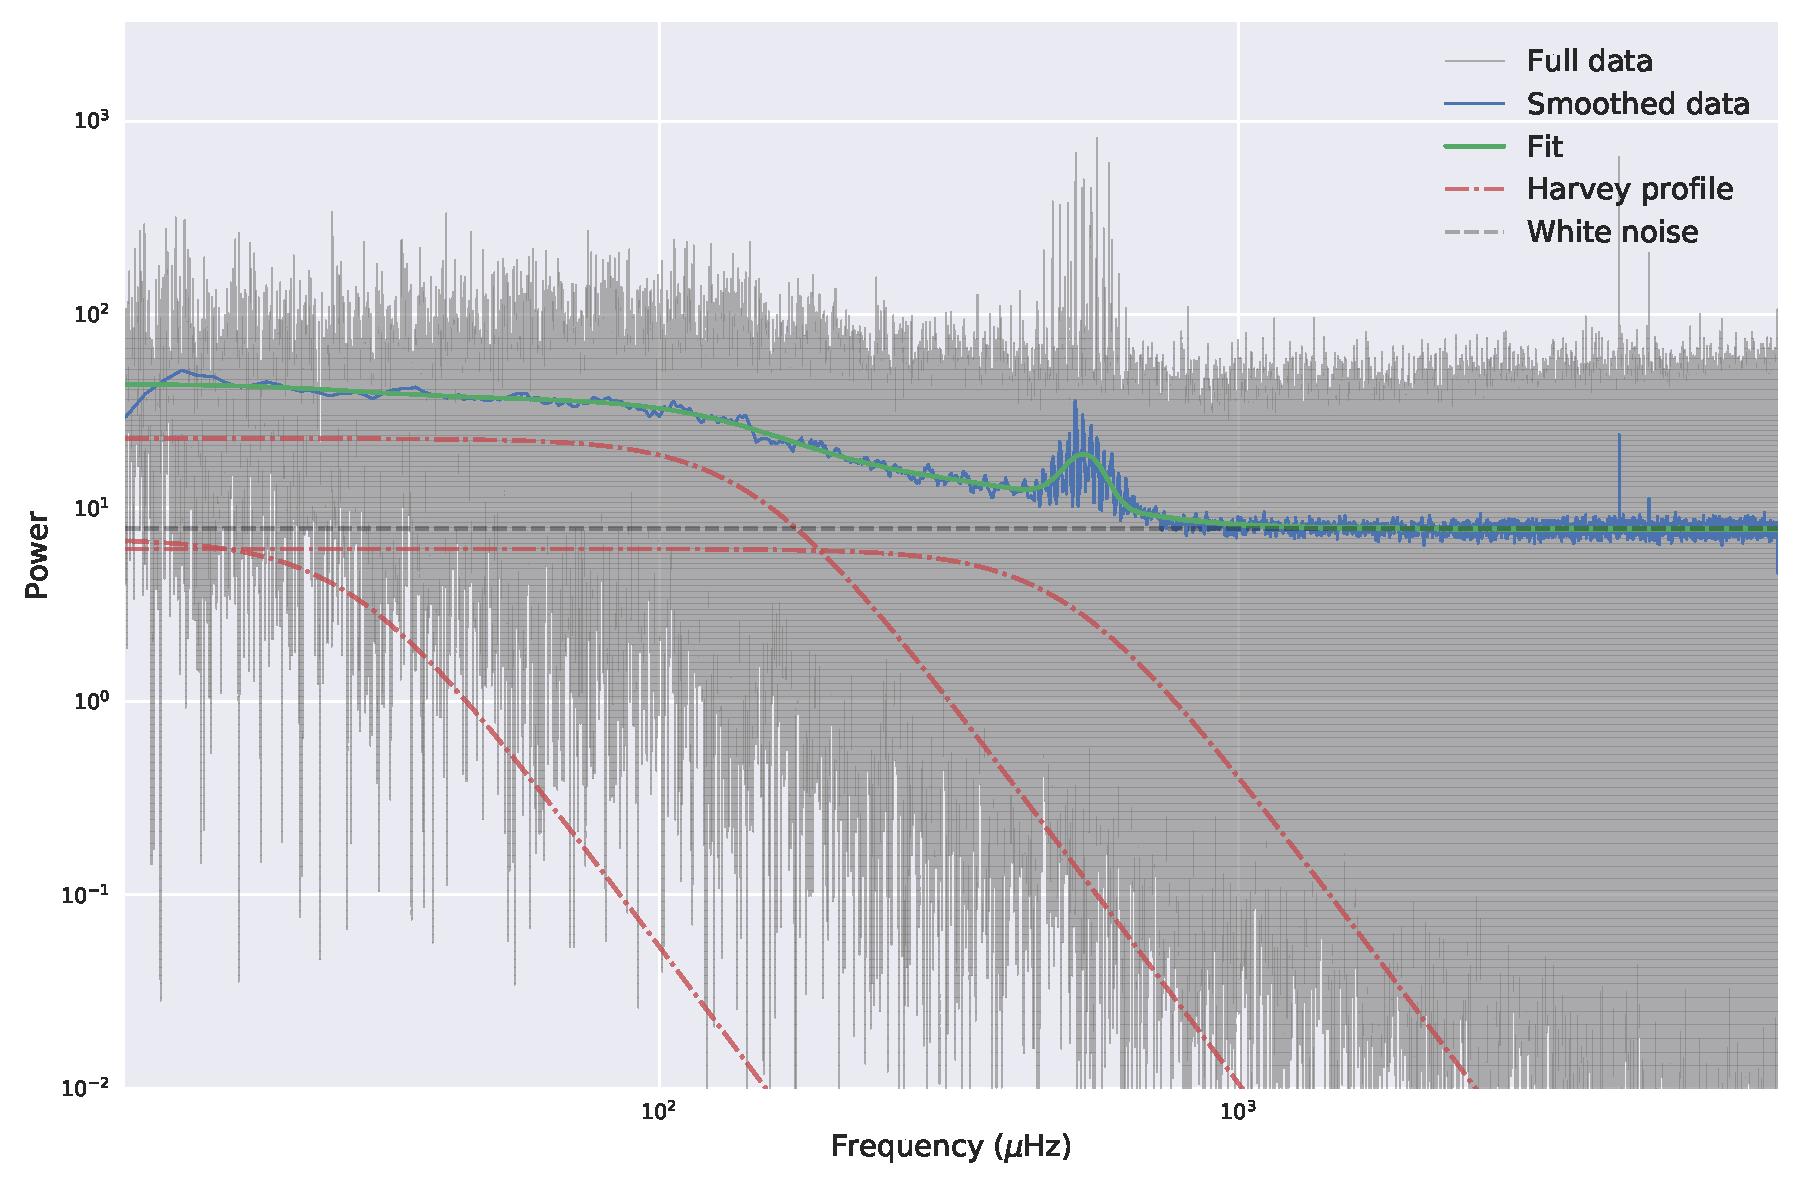
\includegraphics[width=\linewidth]{../figs/psd_fit}
        \caption{The power spectrum data and fit of KIC 7107778 on a log-log scale. The smoothed data has been smoothed using a \SI{6}{\micro Hz} Gaussian 1D Kernel and interpolated to a grid with spacing \SI{0.5}{\micro Hz}. The three Harvey profiles account well for the granulation noise. The peaks to the right are the nyquist frequencies of the short cadence data.}
        \label{fig:envfit}
    \end{figure*}

    \begin{figure*}[th]
        \centering
        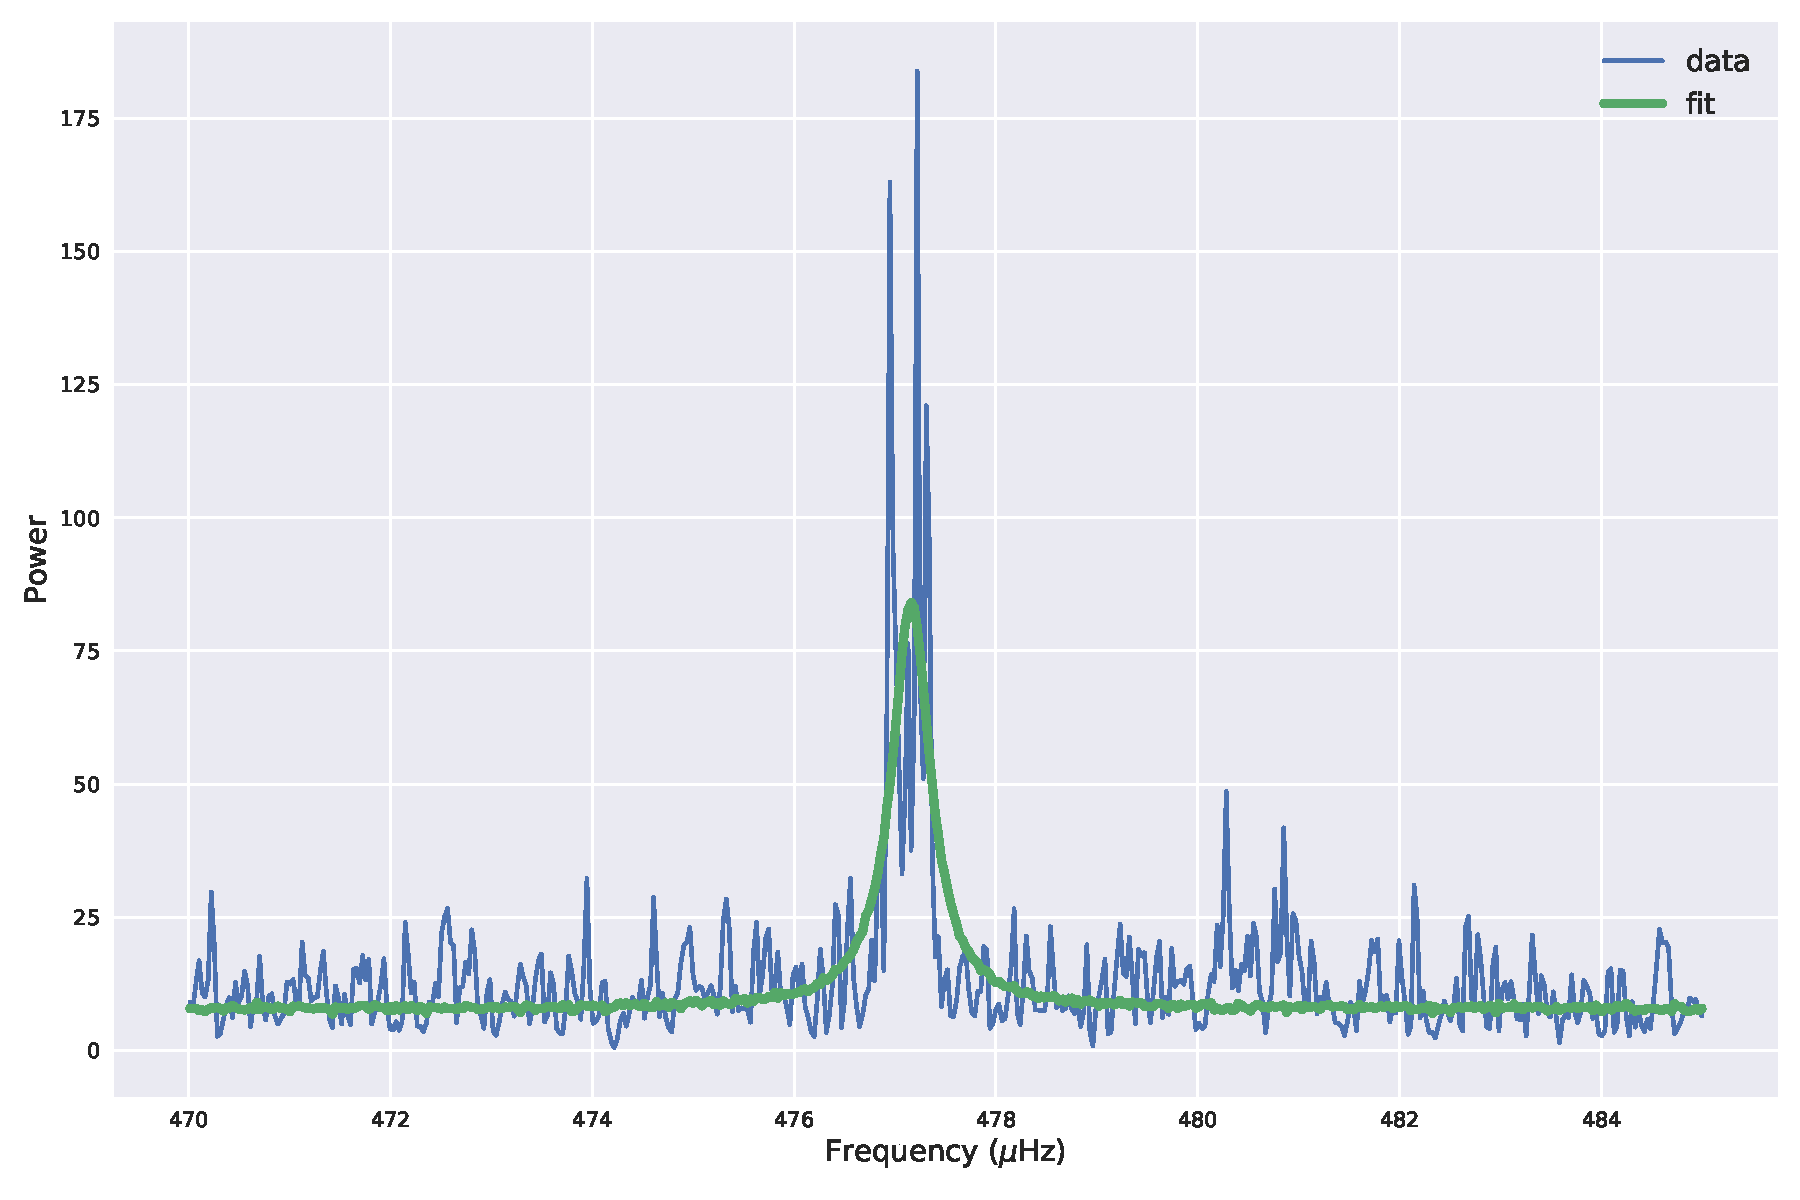
\includegraphics[width=\linewidth]{../figs/mode_fit}
        \caption{The fit of the Lorentzian to a single mode near \SI{477}{\micro Hz}}
        \label{fig:modefit}
    \end{figure*}

    The fits of the Gaussian envelope are shown in \autoref{fig:envfit} and the single oscillation mode fit is shown in \autoref{fig:modefit}. For both fits I took 2000 samples after a 1000 sample burn in. The summary statistics for each posterior are shown in \autoref{tab:envpost} and \autoref{tab:modepost}. One of the parameters of interest for the stellar modeling is $\nu_{max}$, although I am not able to report it because I do not have it split between the two stars effectively. 

    \begin{table}
        \centering
        \caption{Posterior parameters for the Gaussian envelope fit with 95\% HPD interval}
        \label{tab:envpost}
        \begin{tabular}{llllll}
            \hline
                       & Unit              & mean   & sd       & 2.5    & 97.5   \\ \hline\hline
            $a_0$      & $[ppm]$           & 15.15  & 0.4591   & 14.28  & 16.07  \\ 
            $a_1$      & $[ppm]$           & 60.96  & 0.3549   & 60.29  & 61.66  \\ 
            $a_2$      & $[ppm]$           & 59.23  & 0.4772   & 58.32  & 60.17  \\ 
            $b_0$      &  $[\mu Hz]$       & 29.76  & 1.641    & 26.61  & 33.00  \\ 
            $b_1$      & $[\mu Hz]$        & 146.6  & 1.345    & 144.0  & 149.2  \\ 
            $b_2$      & $[\mu Hz]$        & 514.7  & 9.656    & 495.9  & 533.8  \\ 
            $\sigma$   &  $[\mu Hz]$       & 42.57  & 0.9466   & 40.69  & 44.40  \\ 
            $W$        &  $[ppm^2/\mu Hz]$ & 7.808  & 0.01144  & 7.786  & 7.831  \\ 
            $H_0$      & $[ppm/\mu Hz]$    & 29.82  & 0.3629   & 29.10  & 30.53  \\ 
            $\nu_{max}$&$[\mu Hz]$         & 542.2  & 0.8259   & 540.5  & 543.8  \\ 
        \end{tabular}
    \end{table}
   
    \begin{table}
        \centering
        \caption{Posterior parameters for the Lorenztian mode fit with 95\% HPD interval}
        \label{tab:modepost}
        \begin{tabular}{llllll}
            \hline
                     & Unit           & mean   & sd      & 2.5    & 97.5   \\ \hline\hline
            $A$      & $[ppm/\mu Hz]$ & 7.480  & 0.2237  & 7.057  & 7.938  \\
            $\nu_0$  & $[\mu Hz]$     & 477.2  & 0.01817 & 477.1  & 477.2  \\
            $\Gamma$ & $[\mu Hz]$     & 0.2320 & 0.01872 & 0.1948 & 0.2684 \\
        \end{tabular}
    \end{table}


    %-------------------------------------------------------------------------
    \section{Discussion}

    The results of the fitting are not too different from the results of \citet{li}. I cannot conclude any differences because they do not describe their priors at all and I had to interpolate my data. I also cannot comment on the results they receive for the average spacing of modes because I only fit one mode. With that being said, I am very happy with the fact that I was able to fit this model at all given the high dimensionality and modality. The original authors use a completely different package to achieve their samples and I have recreated most of it in python. 

    I wish I could have better computing power or have the time to learn the DIAMONDS package they use for sampling to recreate their analysis. I would say that the authors models effectively work with the data, though.

    %-------------------------------------------------------------------------
    \begin{acknowledgements}
        I would like to thank Dr. Steve Kawaler\footnote{Iowa State University Department of Physics and Astronomy} for his help in understanding the astronomy behind this problem and for his help in accessing the Kepler data I used in the analysis. I would also like to thank Dr. Alicia Carriquiry\footnotemark for her instruction in the ways of Bayesian analysis and Nicholas Berry \footnotemark[\value{footnote}] for his instruction and help with debugging my computational models.

        \footnotetext{Iowa State University Department of Statistics}
    \end{acknowledgements}

    \bibliography{project}
    \appendix*

    %-------------------------------------------------------------------------
    \section{Trace Results}

    \begin{figure*}
        \centering
        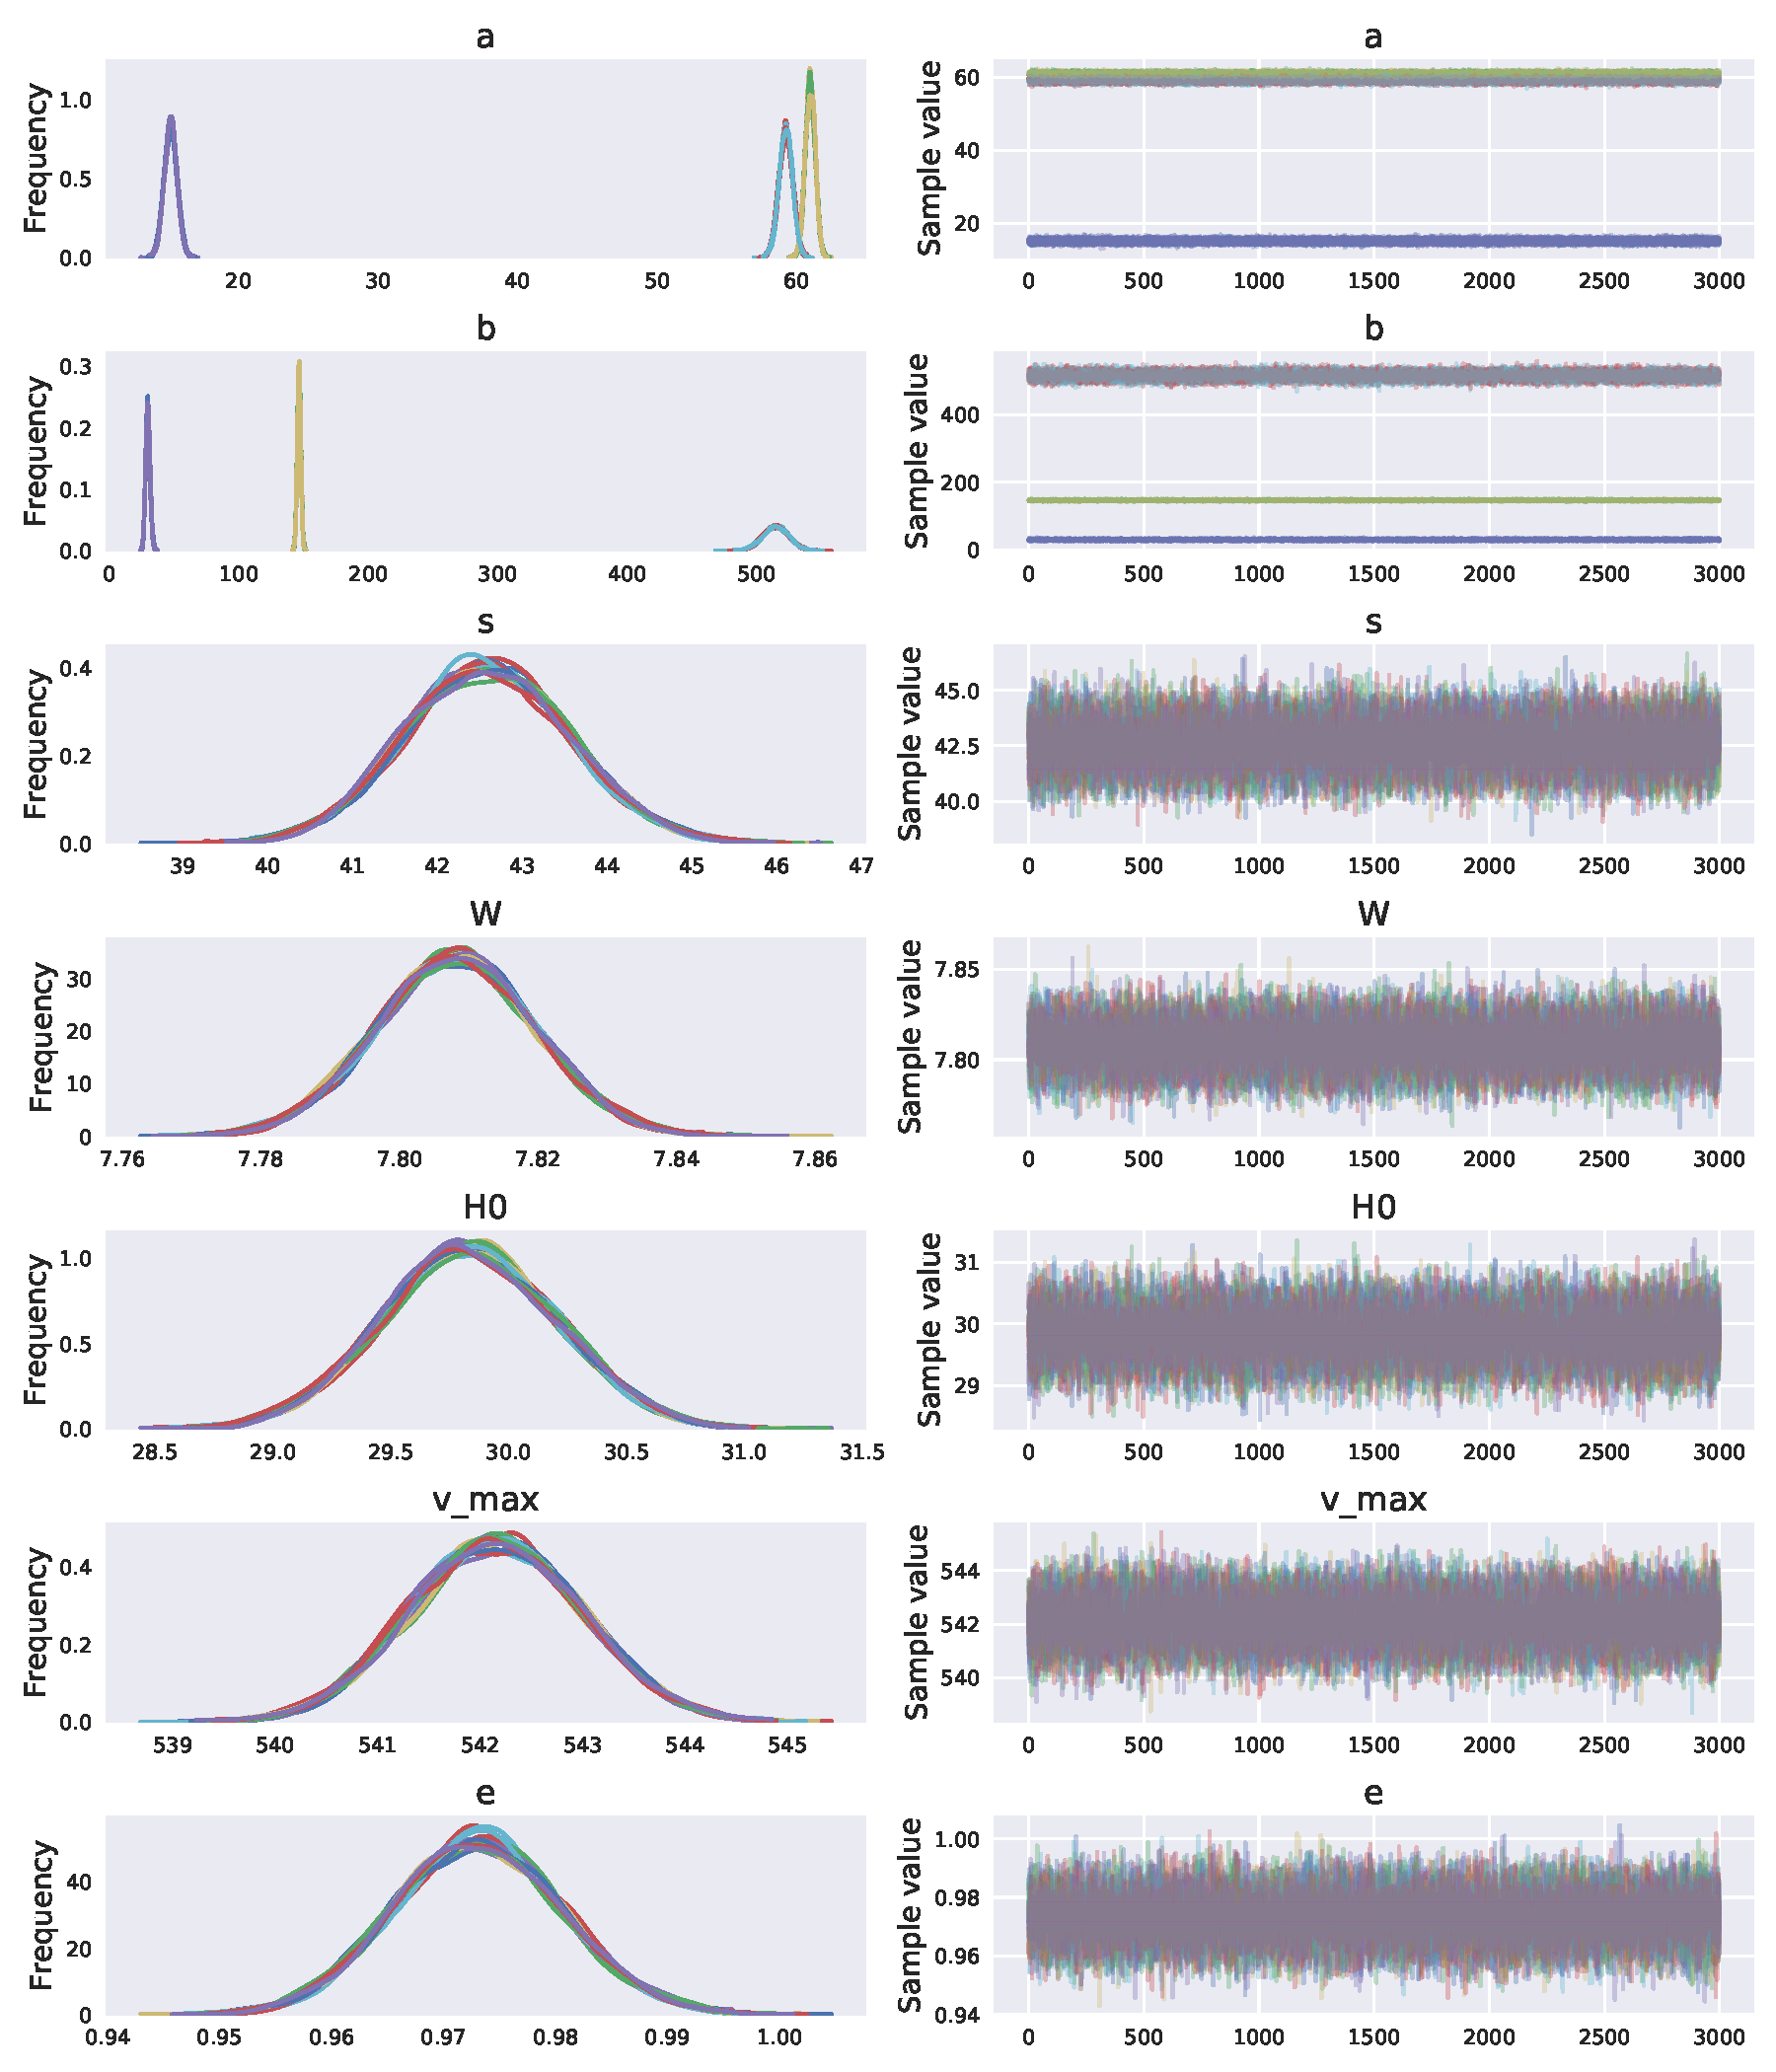
\includegraphics[width=\linewidth]{../figs/trace1}
        \caption{The traces of the envelope fitting.}
        \label{fig:envtrace}
    \end{figure*}

    
    \begin{figure*}
        \centering
        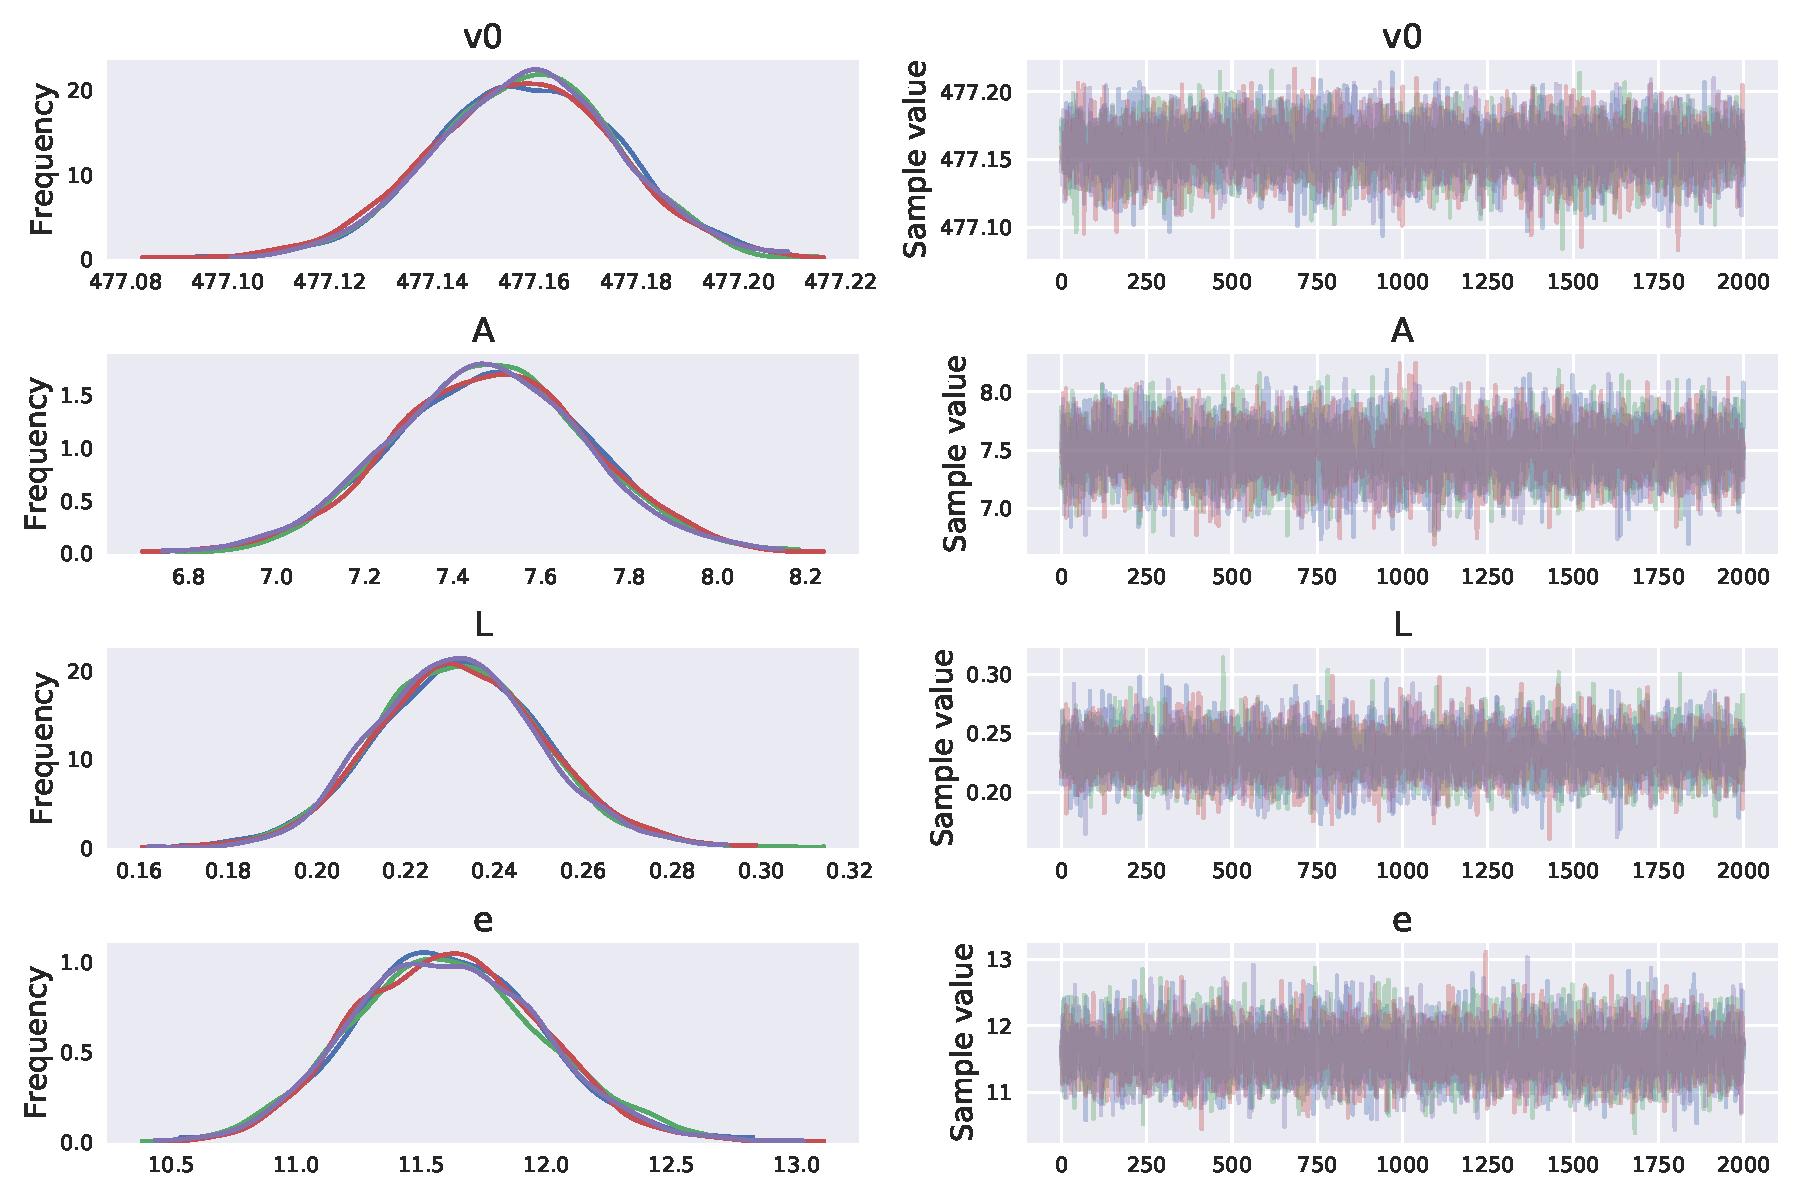
\includegraphics[width=\linewidth]{../figs/mode_trace}
        \caption{The traces of the mode fitting.}
        \label{fig:modetrace}
    \end{figure*}

    

\end{document}